%!TEX root = Main.tex
\documentclass[Main]{subfiles}

\begin{document}

\section{Contribution} % (fold)
\label{sec:contribution}

	The contribution from this mini-project consists of an implementation and test of the DFTSP.
	\subsection{Implementation} % (fold)
	\label{sub:implementation}

		\subsubsection{DFTSP Mote} % (fold)
		\label{sub:dftsp_mote}
			The DFTSP has been implemented on Crossbow Telosb motes\cite{TelosBDatasheet:Online} running the TinyOS\cite{TinyOS:Online} operating system. 
			The DFTSP implementation builds upon the FTSP implementation already available for TinyOS\cite{FTSPImplementationTinyOS:Online}.
			In Figure \ref{fig:nesdoc_dstfp_app_c} a Nesdoc\cite{Nesdoc:Online} overview of the DFTSP application is shown. 
			The application consists of two major components, which each will be described in the following subsections.
			
			\begin{itemize}
			 	\item TimeSyncC - Handles the DFTSP
			 	\item TestResponderC - Handles all test communication
			\end{itemize}

			\begin{figure}[H]
				\centering
				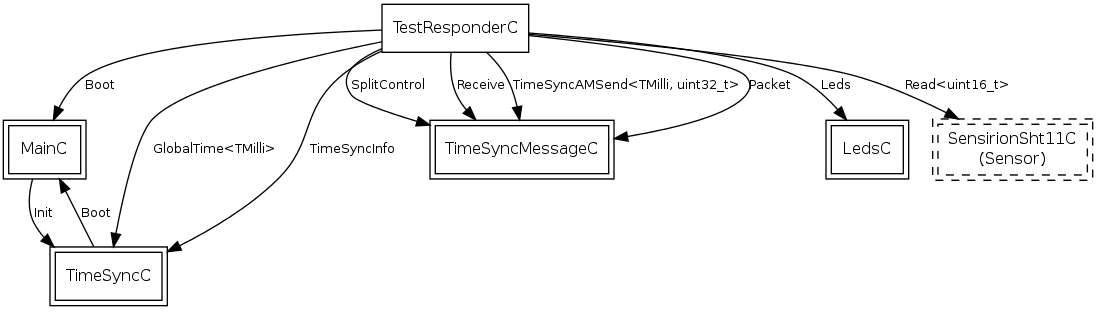
\includegraphics[width=\linewidth]{NesdocDFTSPAppC}
				\caption{DFTSP Application module overview}
				\label{fig:nesdoc_dstfp_app_c}
			\end{figure}

			\paragraph{TimeSyncC} % (fold)
			\label{par:timesyncc}
				The TimeSyncC component was original part of the FTSP implementation, but has been modified and extended to handle the DFTSP.
				In Figure \ref{fig:nesdoc_time_sync_c} an overview of the TimeSyncC component is shown.
				This overview is identical to the FTSP implementation, but the TimeSyncP module have been changed.

				\begin{figure}[H]
					\centering
					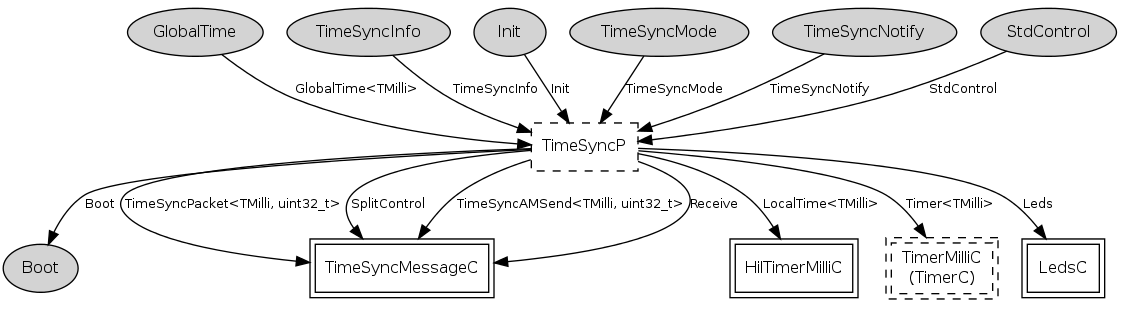
\includegraphics[width=\linewidth]{NesdocTimeSyncC}
					\caption{TimeSyncC module overview}
					\label{fig:nesdoc_time_sync_c}
				\end{figure}

				In DFTSP the parent node must receive broadcast from their children in order to calculate their drift and update its time synchronization period.
				This have numerous impacts on the protocol.

				\textbf{Time Synchronization Message}
				
					The motes needs to include both skew estimation and hop number in the broadcasted time synchronization messages. 
					The hop number is needed, so that the motes can differentiate between parents, children and neighbors. 
					The message is shown in listing \ref{lst:time_sync_msg}.
					\begin{figure}[H]
						\begin{lstlisting}[caption=TimeSyncMsg, style=Code-C, label=lst:time_sync_msg]
		typedef nx_struct TimeSyncMsg
		{
			nx_uint16_t	rootID;		// The node id of the synchronization root
			nx_uint16_t	nodeID;		// The node id of the sender
			nx_uint8_t	seqNum;		// Sequence number for the root
			nx_uint32_t skew;			// Skew 
			nx_uint8_t  hop;			// Hop count from root
			nx_uint32_t	globalTime;
			nx_uint32_t localTime;
		} TimeSyncMsg;
						\end{lstlisting}
					\end{figure}
			
				
				\textbf{Child references}

					The parent must keep reference about its children and their previous skew estimates in order to calculate their drift, since drift is defined as change in skew pr time.
					In listing \ref{lst:child_table} a type definition for a childItem is shown. 
					The childItem contains all the needed information that the parent need to know to calculate the drift of the child.
					The nodeId is used to differentiate between different children.
					The oldTime and oldSkew is needed to calculate the drift and the drift is used to iterate through all children and find the child with the maximum drift, and set the time synchronization period accordingly.

					To store multiple children a table of childItems was defined with a constant size. Depending on the application, the table size could vary a lot and should possibly be of dynamic size.

					\begin{figure}[H]
						\begin{lstlisting}[caption=Child table, style=Code-C, label=lst:child_table]
		typedef struct ChildItem {
			uint16_t nodeId;
			uint32_t oldTime;
			float oldSkew;
			float drift;
		} ChildItem;

		ChildItem childTable[MAX_CHILDREN];
			    		\end{lstlisting}
			    	\end{figure}
			    
			    \newpage
			    \textbf{Child message handling}	

			    	Since the TimeSyncMsg contains the hop number all received messages are compared with the motes own hop count, and if the hop count is smaller, then the message is assumed to be a child broadcast.
			    	In listing \ref{lst:child_handling} the handling of incoming child messages is shown.
			    	If the child exists in the childTable the drift is calculated and the maximum drift for all children is found and used to update the time synchronization period.
			    	Otherwise the child is added to the table.
			    	\begin{figure}[H]
						\begin{lstlisting}[caption=Handling incoming child msg, style=Code-C, label=lst:child_handling]
void handleNewChildSkew(TimeSyncMsg *msg) {
	uint8_t i, childExist = 0;
	float maxDrift = 0;
	for(i = 0; i < childEntries; i++)
	{
		if(childTable[i].nodeId == msg->nodeID)
		{
			float skewChange = 0, drift = 0;
			int32_t timeSinceLastSkew = 0;
			childExist = 1;
			
			skewChange = u2f(msg->skew) - childTable[i].oldSkew;				
			if(skewChange < 0)
			{
				skewChange = -skewChange; // unit is [ms/s]
			}
			
			timeSinceLastSkew = (msg->localTime - childTable[i].oldTime); // unit is [ms]
			if(timeSinceLastSkew != 0) {
				drift = (skewChange*1000)/timeSinceLastSkew;	// unit is [ms/s^2]
			}
			childTable[i].drift = drift;
			childTable[i].oldSkew = u2f(msg->skew);
			childTable[i].oldTime = msg->localTime;					
		}
		
		if(childTable[i].drift > maxDrift)
			maxDrift = childTable[i].drift;
	}
	if(childExist == 0)
	{
		if(childEntries < MAX_CHILDREN)
		{
			childTable[childEntries].nodeId = msg->nodeID;
			childTable[childEntries].oldSkew = u2f(msg->skew);
			childTable[childEntries].oldTime = msg->localTime;
			childEntries++;
		}
	} else {
		updateBeaconPeriod(maxDrift);
	}
}

						\end{lstlisting}
			    	\end{figure}

			    \newpage
			    \textbf{Calculate time synchronization period}

			    	As described in \cite{dynamicFTSParticle}, the calculation of the time synchronization period is a resource consuming process, since it contains a square root calculation.
			    	This calculation is instead performed as shown in listing \ref{lst:time_sync_calc}.
			    	This reduced the computational effort, but limits the precision of the period to a discrete number. 
			    	It is chosen to increase the period with steps of 10 seconds, and limit it to maximum 255 seconds.
			    	
					\begin{figure}[H]
						\begin{lstlisting}[caption=Calculate time synchronization period, style=Code-C, label=lst:time_sync_calc]
		void updateBeaconPeriod(float maxDrift)
	    {
	    	float error = 0, tau = MIN_BEACON_INTERVAL;
	    	float c = 10;
	    	if(maxDrift != 0)
	    	{
	    		while(error < OFFSET_ERROR_BOUND)
	    		{
	    			tau = tau + c;
	    			error = maxDrift*1000*((tau*tau)/2);
				}
				
				if(tau < MIN_BEACON_INTERVAL)
					tau = MIN_BEACON_INTERVAL;
				else if(tau > MAX_BEACON_INTERVAL)
					tau = MAX_BEACON_INTERVAL;
					
				atomic beaconPeriod = (unsigned char)(tau);
	    	}
	    }
			    		\end{lstlisting}
			    	\end{figure}			

				\textbf{Testing changes}

					In order to test the performance of the DFTSP the TestResponderC module must be able to access both the drift and synchronization period from the motes. 
					The existing TimeSyncInfo interface have been extended so that both variables is accessible.


			% paragraph timesyncc (end)

			

			
			\newpage
			\paragraph{Test Responder Module} % (fold)
			\label{par:test_responder_module}
				The test responder module has been added to the DFTSP application to enable it to participate in the tests.
				An overview given in Figure \ref{fig:DFTSPResponderOverview} shows the modules used.

				\begin{figure}[H]
					\centering
					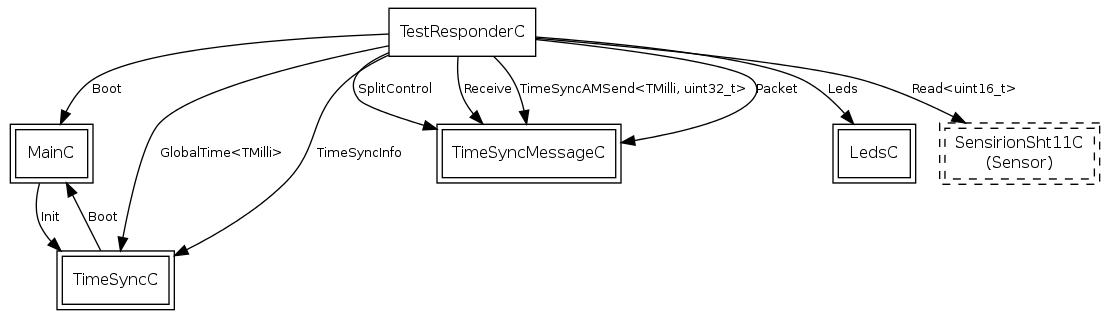
\includegraphics[width=\linewidth]{DFTSPResponderOverview.png}
					\caption{DFTSP Responder Module Overview}
					\label{fig:DFTSPResponderOverview}
				\end{figure}

				The responsibility of the test responder module is to receive the query message from the broadcaster, acquire the necessary data and respond to the broadcaster.
				The data is shown in listing \ref{code:test_data}.

				\begin{figure}[H]
					\begin{lstlisting}[caption=DFTSP Test Data, style=Code-C, label=code:test_data]
		typedef nx_struct SyncReportMsg
		{
			nx_uint16_t	nodeID;			// the node if of the sender
			nx_uint32_t	globalTimeEst;	// the senders estimation of the global time
			nx_uint8_t  syncPeriod;		// the senders synchronization period
			nx_uint32_t  drift;			// the senders estimation of its child's drift
			nx_uint16_t  temp;			// the senders temperature measurement
			nx_uint8_t	seqNum;		// sequence number for the root
		} SyncReportMsg;

					\end{lstlisting}
				\end{figure}

				All fields except the $temp$, which holds the temperature of the mote, are provided by the DFTSP module.
				The temperature is read using the Sensirion SHT11\cite{tempSensorDatasheet} temperature and humidity sensor on the Telosb.
				The module connection, read invoke and readDone event are shown in listing \ref{code:temp_impl}.

				hvornår læser den tempen?

				\begin{figure}[H]
					\begin{lstlisting}[caption=Temperature reading implementation, style=Code-C, label=code:temp_impl]
		typedef nx_struct SyncReportMsg
		{
		// Temperature Module Connection
		components new SensirionSht11C() as Sensor;
		App.Read -> Sensor.Temperature;

		// Read invoke
		event message_t* Receive.receive(message_t* msgPtr, void* payload, uint8_t len)
		{
	    	call Read.read();
	    	// Rest of the receive implementation


		// ReadDone event
		event void Read.readDone(error_t result, uint16_t val)
		{
			if(result == SUCCESS)
			temp = val;
		}

						\end{lstlisting}
				\end{figure}
			% paragraph test_responder_module (end)
		% subsubsection dftsp_mote (end)
		
		
		\subsubsection{Broadcaster Mote} % (fold)
		\label{sub:broadcaster_mote}
			The broadcaster application has also been implemented on a Crossbow Telosb mote. 
			An overview of the application given in Figure \ref{fig:broadCastAppOverview} shows the modules used. 

			\begin{figure}[H]
				\centering
				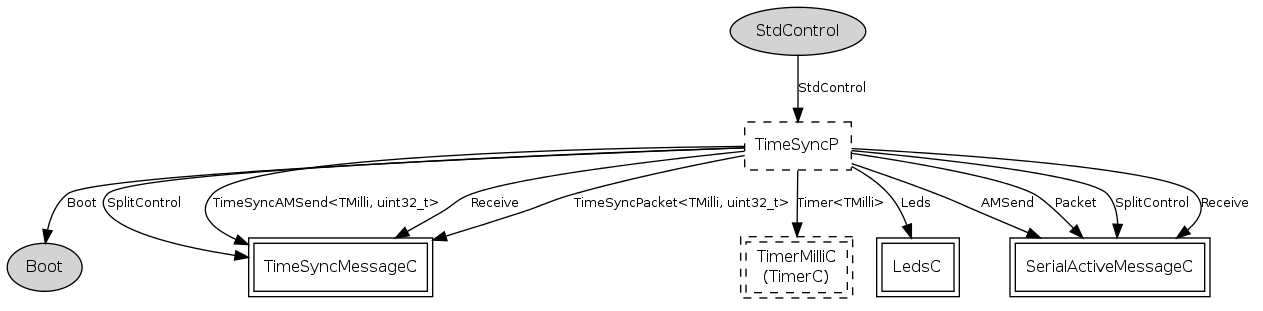
\includegraphics[width=\linewidth]{BroadcastAppOverview.png}
				\caption{Broadcast application overview}
				\label{fig:broadCastAppOverview}
			\end{figure}

			The broadcaster application is also based on the FTSP implementation given in \cite{FTSPImplementationTinyOS:Online}.	
			Periodically, at the $BROADCAST\_RATE$, the broadcaster mote will query the DFTSP parent and child for the data shown in listing \ref{code:test_data}.
			Upon reception, the broadcaster application sends the data to the test PC using a USB connection, as seen in Figure \ref{fig:TestSetup}.

		% subsubsection broadcaster_mote (end)
	

		
		\subsubsection{Serial Java Application} % (fold)
		\label{sub:serial_java_application}
			The Serial Java Application is responsible for receiving test data from the broadcaster mote and writing the data to a text file.
			The data is formatted appropriately prior to graphing in Matlab for presentation.
			Furthermore the actual temperature is calculated from the temperature sensor output.
			The temperature was calculated with the following formula\cite{tempSensorDatasheet}:

			\begin{equation}
			T = d_1 + d_2 * SO_T
			\end{equation} 

			The values used to obtain the temperature $T$ from the sensor ouput $SO_T$:
			\begin{equation}
			d_1 = -39,6\ \ \ d_2 = 0,01
			\end{equation} 

			Figure \ref{fig:JavaTextOutput} shows how an output file is formatted.
			The columns represent from left to right: NodeID, Global Time Estimate, Synchronization Period, Drift/Skew, Temperature, DFTSP sequence number and Serial Java application time stamp.
			
			In figure \ref{fig:JavaTextOutput} the parent has NodeID 1 and the child has NodeID 3.
			The synchronization period is 40 seconds, whereas the 10 seconds from the child should be disregarded as the child does not have any children of it's own.
			The fourth column shows either skew or drift depending on whether the data comes from the child or parent respectively.
			The DFTSP sequence number is not incremented in the figure because the broadcast rate is much smaller than the DFTSP synchronization period.
			The final column with the Serial Java time stamp is used to pair data entries from the same broadcast round to be able to calculate the global time estimation error.

			\begin{figure}[H]
				\centering
				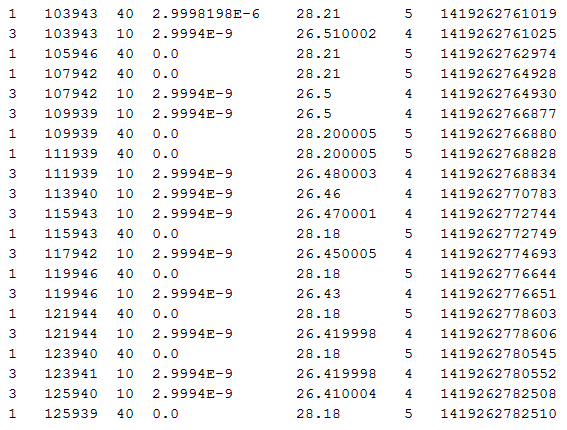
\includegraphics[width=0.5\linewidth]{JavaTextOutput.png}
				\caption{Serial Java Application text output}
				\label{fig:JavaTextOutput}
			\end{figure}

			
		% subsection serial_java_application (end)

	% subsection implementation (end)

	\subsection{Test Setup} % (fold)
	\label{sub:test_setup}

		As seen in figure \ref{fig:TestSetup} the test setup consisted of the following items:

		\begin{itemize}
			\item Parent mote
			\item Child mote
			\item Broadcaster mote
			\item Test PC
			\item Blow dryer 
		\end{itemize}

		The broadcaster mote is connected to the test PC with a USB cable.
		The child mote is placed in front of the blow dryer which is used to simulate an unstable environment.
		The parent node is placed in the vicinity of the other motes to avoid dropped packages due to range issues.

		\begin{figure}[H]
			\centering
			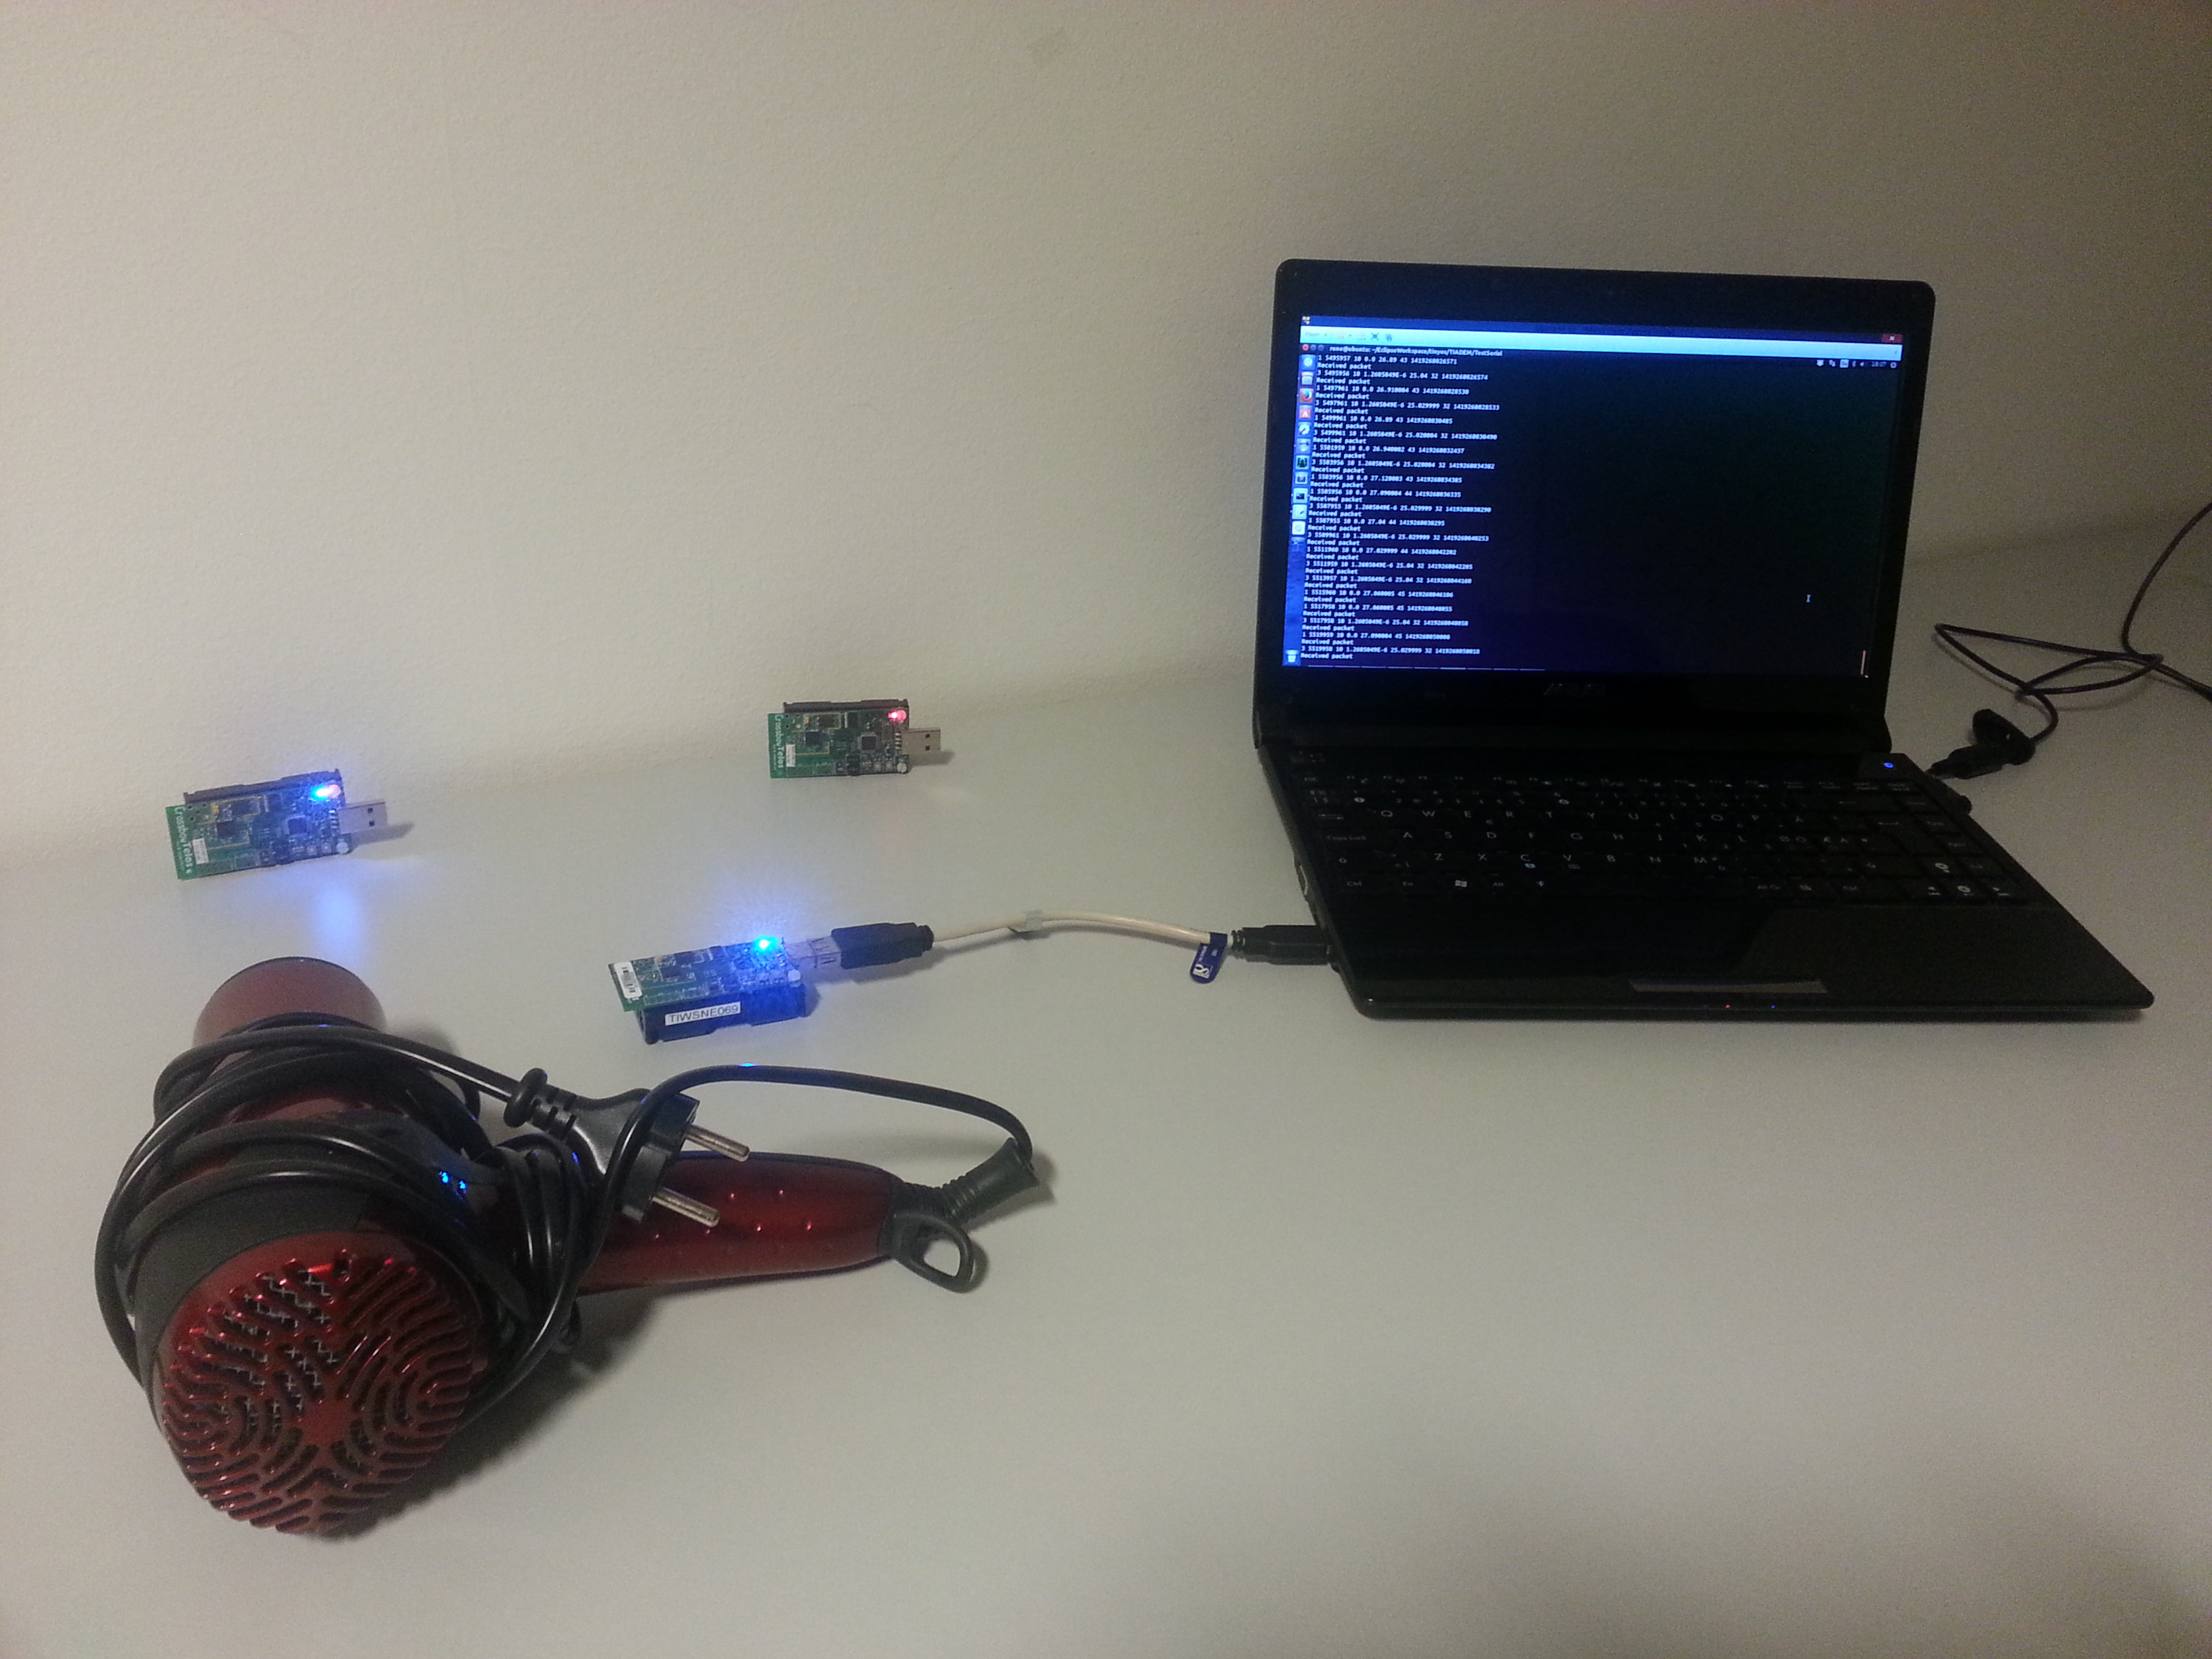
\includegraphics[width=\linewidth]{TestSetup.jpg}
			\caption{Test Setup}
			\label{fig:TestSetup}
		\end{figure}

		\subsubsection{Test Parameters} % (fold)
		\label{subsub:test_parameters}
			The tests were performed with the following parameters:

			\begin{itemize}
				\item Parent mote id set to 1
				\item Child mote id set to 3
				\item Synchronization period range limited to 10-255 seconds spaced by 10 seconds
				\item Broadcast rate set to 2 seconds
				\item The average error bound is set to 2 ms
			\end{itemize}

			The tests were performed in two different environments.
			In the stable environment the temperature of the motes is not actively raised or lowered.
			In the unstable environment the temperature of the child mote is raised with the blow dryer and lowered by placing the mote outside.
		
		% subsubsection test_parameters (end)
	
	% subsection test_setup (end)

	\subsection{Test Results} % (fold)
	\label{sub:test_results}
		The test results are split into results from a stable environment and an unstable environment.  


		\subsubsection{Stable Environment} % (fold)
		\label{sub:stable_environment}
			
			
			Figure \ref{fig:stableSynchronization} shows the results from the test in a stable environment.
			\\The temperature remains approximately constant whilst the synchronization error remains under the average error bound.
			The synchronization period is quickly set to the maximum allowed value of 255 seconds. This indicates that the drift calculated by the parent mote has been 0 for the duration of the test.   

			\begin{figure}[H]
				\centering
				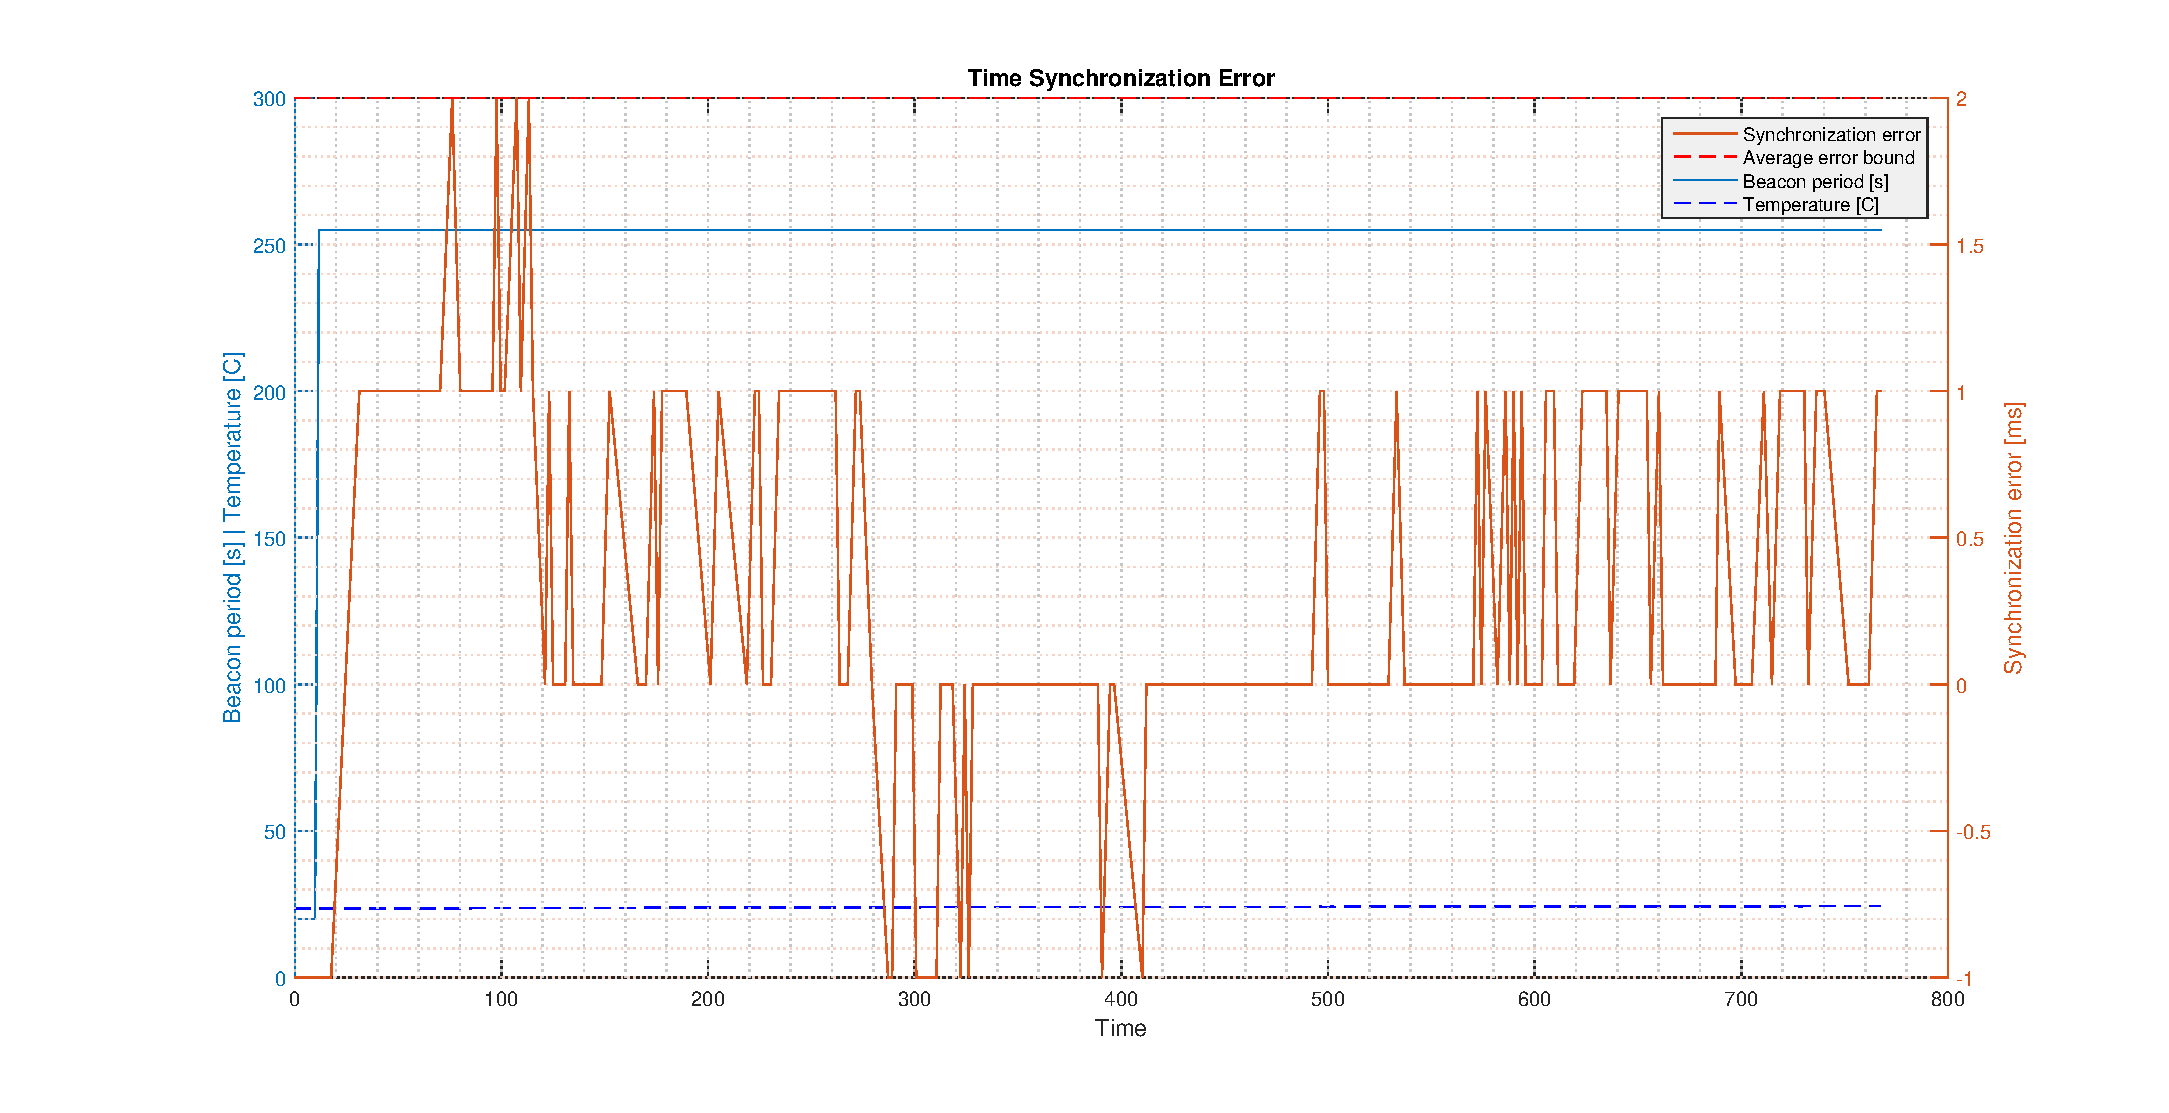
\includegraphics[width=\linewidth]{StableSynchronization.eps}
				\caption{Stable Environment Test Results}
				\label{fig:stableSynchronization}
			\end{figure}

			The DFTSP behaves as expected under these good conditions with no drift. 
			The synchronization error remains below the bound even though the synchronization period is large, since the skew estimate in the child holds.
			\\ In this case, the DFTSP behaves very similarly to the ordinary FTSP, since there is little need for dynamic behavior. 


		% subsubsection stable_environment (end)

		\subsubsection{Unstable Environment} % (fold)
		\label{sub:unstable_environment}
			
			 Figure \ref{fig:unstableSynchronization} shows the results from the test in an unstable environment.
			 \\The temperature of the child mote is kept constant for the first approximately 400 seconds.
			 The synchronization error is similar to the stable case, however the synchronization period rises somewhat slower.
			 This indicates that some drift was present at the beginning of the test, even though the temperature was constant. 

			 A clear correlation between synchronization error and temperature is seen when the temperature is raised.
			 660 seconds into the test, the synchronization period is drastically reduced, leading to an instantaneous reduction in the error.
			 This showcases the principle behind adjusting the synchronization period dynamically in order to obtain the average error level.

			 As the temperature stabilizes towards the end of the test, the error is lowered and the synchronization period returns to the maximum value.  

			\begin{figure}[H]
				\centering
				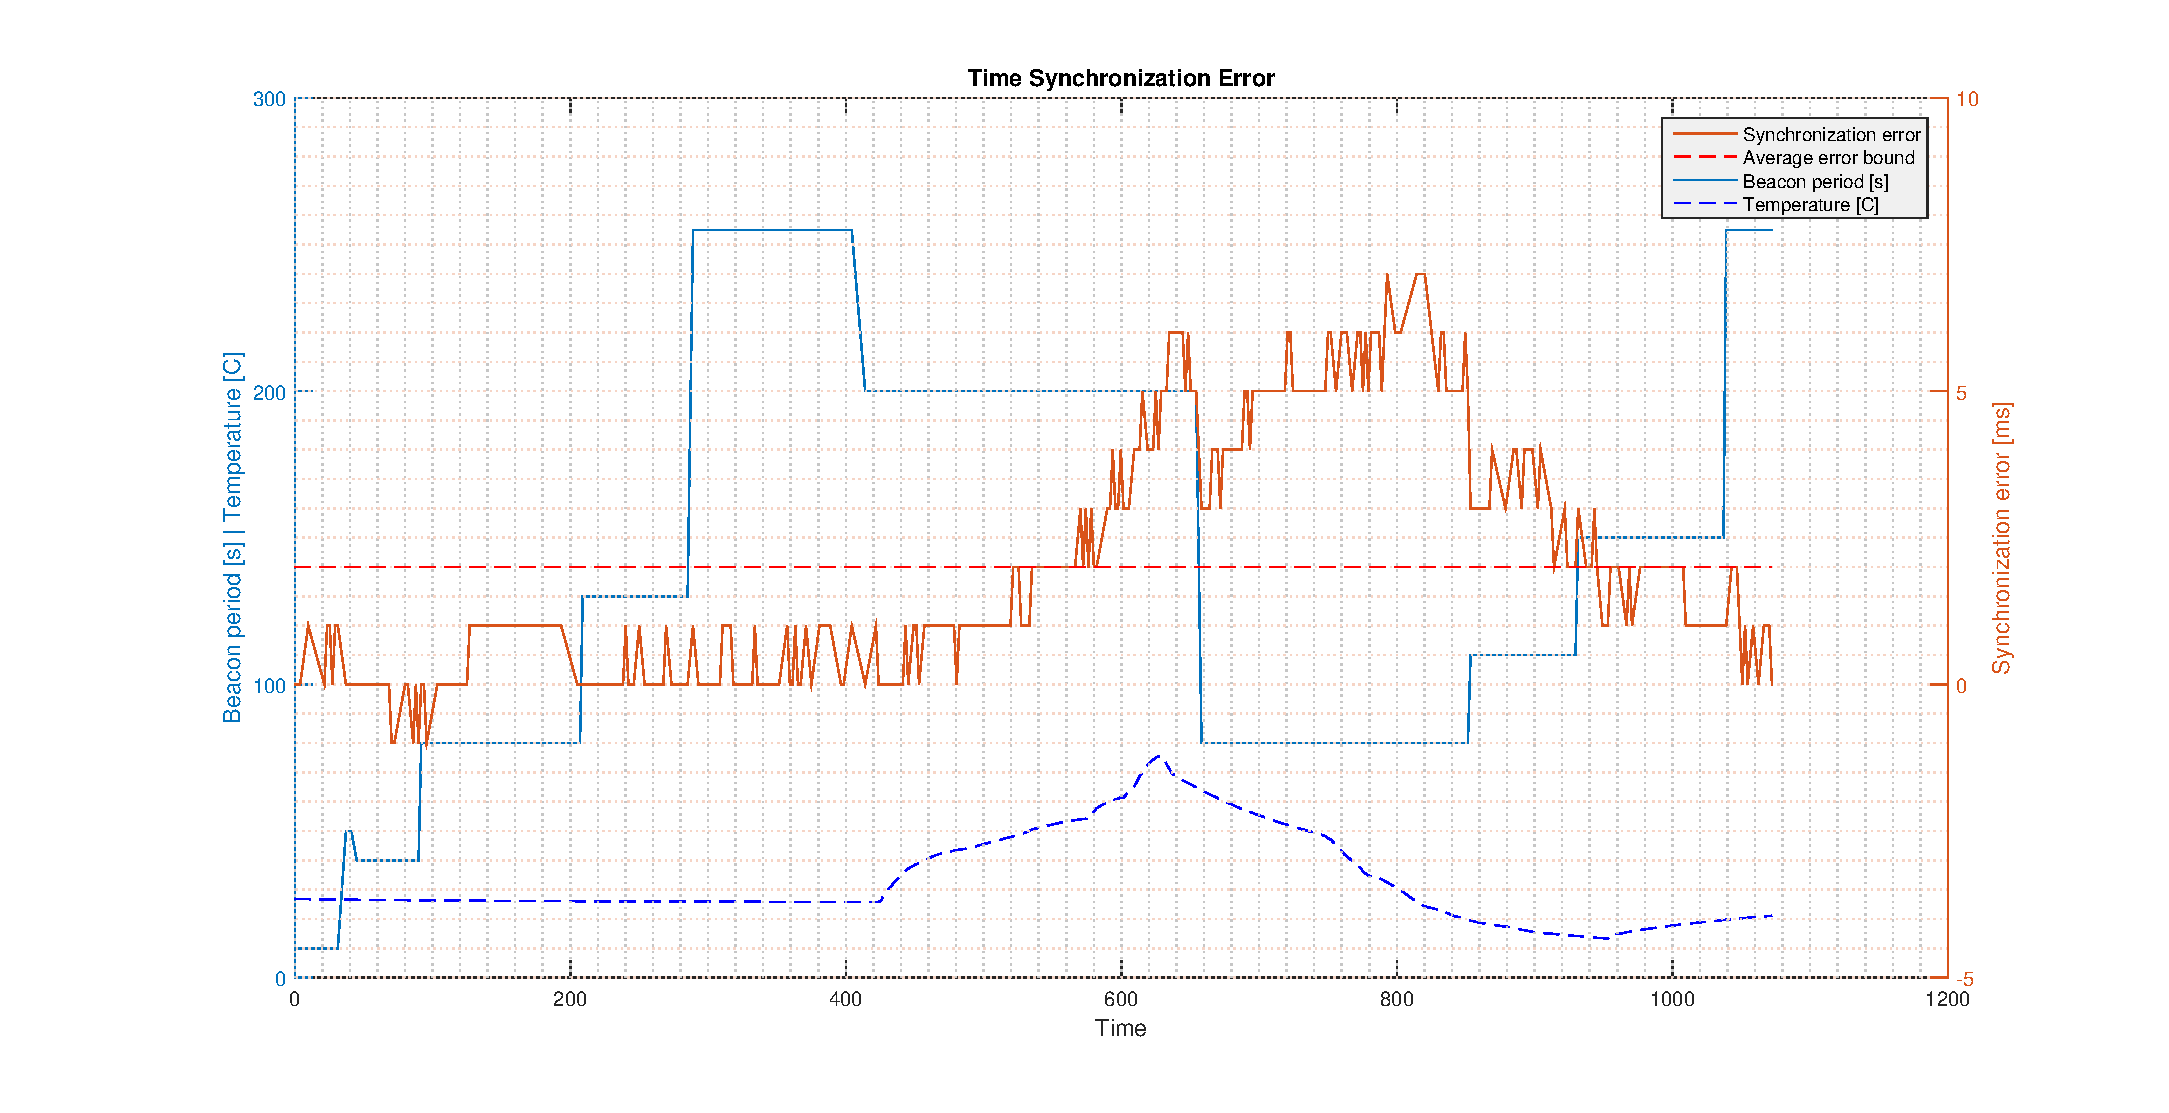
\includegraphics[width=\linewidth]{Synchronization.eps}
				\caption{Unstable Environment Test Results}
				\label{fig:unstableSynchronization}
			\end{figure}

			The correlation between temperature change and synchronization error is evident from the skew/temperature plots of figure \ref{fig:SkewunStable}.
			The temperature changes lead to an increase in the skew.
			This plot further clarifies the drastic drop in synchronization period at 660 seconds.
			The synchronization period is dependent on the drift, which is skew change. 
			Hence the period is lowered when the drift changes drastically, as it does at 660 seconds.


			\begin{figure}[H]
				\centering
				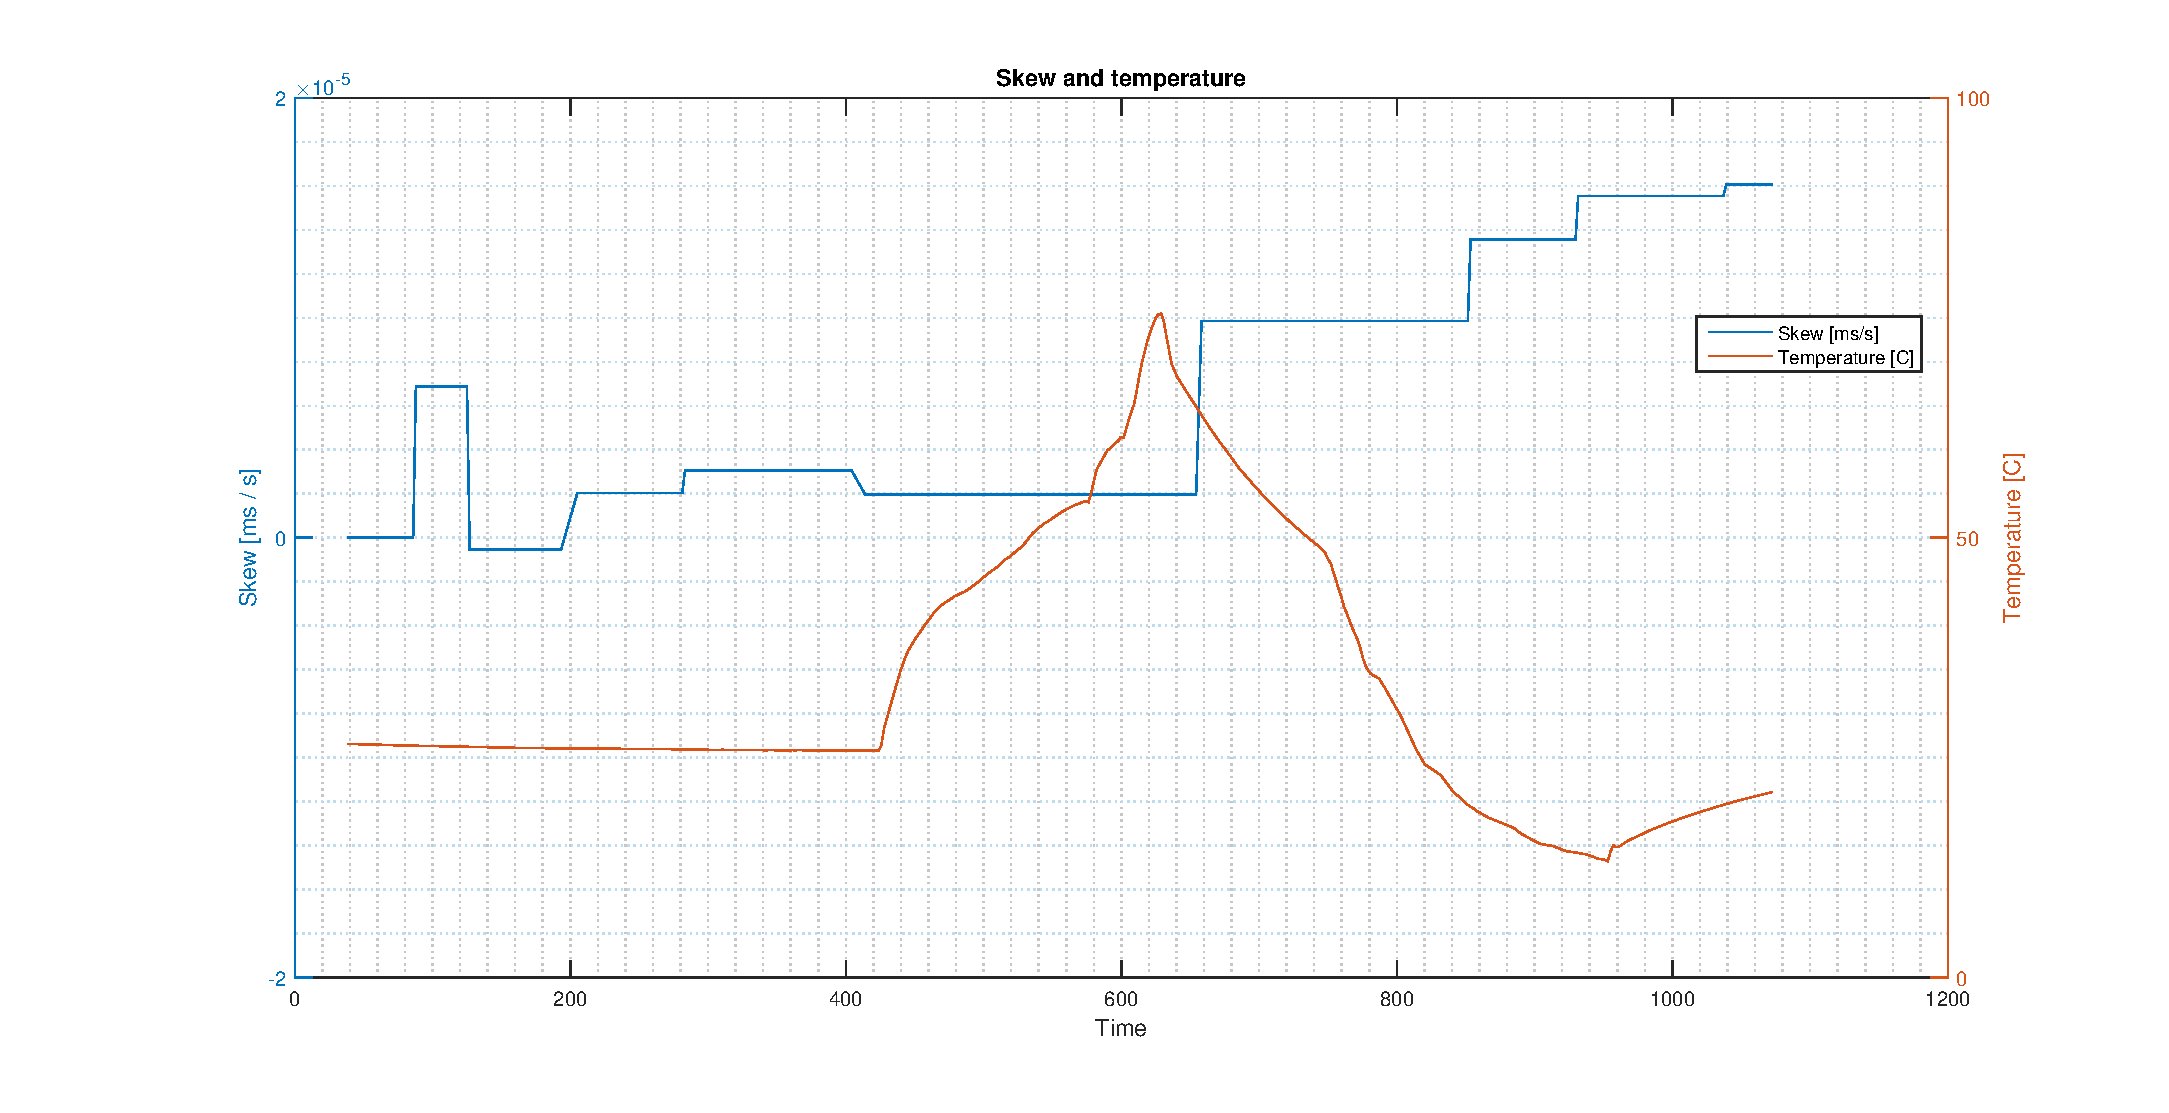
\includegraphics[width=\linewidth]{SkewUnstable.eps}
				\caption{Clock Skew and Temperature in Unstable Environment}
				\label{fig:SkewunStable}
			\end{figure}

			The results show that the DFTSP algorithm successfully adjust the synchronization period during periods of both high and low clock drift.  

		% subsubsection unstable_environment (end)
	
	% subsection test_results (end)

% section contribution (end)

\end{document}
